

% Summary semiconductor devices D-ITET
% ===========================================================================
% @Author: Noah Huetter
% @Date:   2019-02-20 17:26:28
% @Last Modified by:   noah
% @Last Modified time: 2019-03-13 15:26:54
% ---------------------------------------------------------------------------

\documentclass[a4paper, fontsize=8pt, landscape, DIV=1]{scrartcl}
\usepackage{lastpage}
\usepackage{hyperref}
% Include general settings and customized commands
%
% General packages and settings
% ===========================================================================
% Author:			Silvano Cortesi (cortesis@student.ethz.ch)
% Version:			1.2
% Last changed:		03.01.2018
%
% ---------------------------------------------------------------------------




\usepackage[german]{babel} %choose your language \usepackage[german]{babel}
%\usepackage[T1]{fontenc}
\usepackage[utf8]{inputenc}
\usepackage{fancyhdr}
%\usepackage{lastpage}
%\usepackage{lmodern}
\usepackage{enumerate}
%\usepackage{float} % for positioning of figures
\usepackage[landscape, margin=1cm]{geometry}
\usepackage[dvipsnames]{xcolor}
\usepackage{pdfpages}


%% Math %%
\usepackage{todonotes}
\usepackage{amscd}
\usepackage{blindtext}
\usepackage{enumitem}
\usepackage{multicol}
\usepackage{parskip}
\usepackage{empheq}
\usepackage{amsmath}
\usepackage{amsfonts}
\usepackage{amssymb}
\usepackage{amsthm}
%\usepackage{dsfont}
%\usepackage{esint} % provides \oiint
\usepackage{mathrsfs}
%\usepackage{trfsigns}
%\numberwithin{equation}{subsection}
%\usepackage{numprint}

%% Graphics & Charts %%
\usepackage{graphicx}
%\usepackage{pdfpages}
%\usepackage{booktabs}
\usepackage{array}
%\usepackage{paralist}
%\usepackage{framed}
%\usepackage{trfsigns}
\usepackage{tikz}
%\usepackage[lofdepth,lotdepth]{subfig}
%\usepackage{tikz}  %Graphen zeichnen
%\usetikzlibrary{decorations.pathmorphing}
%\usetikzlibrary{arrows.meta,arrows}
%\usepackage{pgfplots}
%% General Settings %%
%\setlength{\parindent}{0px}
%\setkomafont{captionlabel}{\normalfont\bfseries}

%\pagestyle{fancy}
%\lfoot{\tiny \today}
%\rfoot{\thepage\  / \pageref{LastPage}}
%\cfoot{}
%\renewcommand{\footrulewidth}{0.4pt}

%% provides command \uline{} for underlining words
%\usepackage{ulem}

%% colour headings
%\usepackage{color}
%\definecolor{bluen}{cmyk}{1,0.5,0,0}
%\definecolor{bloodorange}{cmyk}{0,.92,1,.2}
%\addtokomafont{section}{\color{bloodorange}}
%\addtokomafont{subsection}{\color{bloodorange}}
%\addtokomafont{subsubsection}{\color{bloodorange}}
%\addtokomafont{paragraph}{\small\color{bloodorange}}
%\addtokomafont{subparagraph}{\small\color{bloodorange}}

%% Signs & Special Formating %%
%\usepackage{ulem} %normalem: \emph{Text} is italic again.
%\usepackage{multicol,multirow}
%\usepackage{tabularx}
%\usepackage{stackrel}
%\usepackage{makeidx}
%\usepackage{mparhack} % bessere margiale bei seitenumbruch

% make document compact
\usepackage[compact]{titlesec}
\titlespacing{\section}{0pt}{*0}{*0}
\titlespacing{\subsection}{0pt}{*0}{*0}
\titlespacing{\subsubsection}{0pt}{*0}{*0}

\parindent 0pt
\pagestyle{empty}
\setlength{\unitlength}{1cm}
\setlist{leftmargin = *}

%include also newer PDF
\pdfminorversion=6

% Set the color of your style
% Avaiable are: Apricot, Aquamarine, Bittersweet, Black, Blue, blue, BlueGreen, BlueViolet, BrickRed, Brown, BurntOrange, CadetBlue, CarnationPink, Cerulean, CornflowerBlue, Cyan, Dandelion, DarkOrchid, Emerald, ForestGreen, Fuchsia, Goldenrod, Gray, Green, GreenYellow, JungleGreen, Lavender, ... (more at: http://en.wikibooks.org/wiki/LaTeX/Colors)
\def\StyleColor{MidnightBlue}

%
% General commands
% ===========================================================================
% Author:			Silvano Cortesi (cortesis@student.ethz.ch)
% Version:			1.2
% Last changed:		03.01.2018
%
% ---------------------------------------------------------------------------

%..ROEMISCHE_ZAHLEN
	\newcommand{\Roe}[1]{\uppercase\expandafter{\romannumeral #1 }}

%..ZAHLENMENGEN
	\newcommand{\N}{\mathbb{N}}
	\newcommand{\Z}{\mathbb{Z}}
	\newcommand{\Q}{\mathbb{Q}}
	\newcommand{\R}{\mathbb{R}}
	\newcommand{\real}{\R}
	\newcommand{\C}{\mathbb{C}}
	\newcommand{\complex}{\C}
	\newcommand{\0}{\mathbb{O}}
	\newcommand{\F}{\mathbb{F}}
	\newcommand{\K}{\mathbb{K}}
    \newcommand{\angstrom}{\textup{\AA}}
    
%..PFEILE
	\renewcommand{\leadsto}{\Longrightarrow}
	\newcommand{\leftrightleadsto}{\Longleftrightarrow}

%..VEKTOREN
	\newcommand{\Ul} {\underline}
	\newcommand{\vEx} {\vec{e}_x}
	\newcommand{\vEy} {\vec{e}_y}
	\newcommand{\vEz} {\vec{e}_z}
	\newcommand{\vEq} {\vec{e_1}}
	\newcommand{\vEw} {\vec{e_2}}
	\newcommand{\vEe} {\vec{e_3}}
	\newcommand{\transpose} {^{\text{T}}}
	\newcommand{\vect}[1]{\boldsymbol{#1}}
	
%..MATRIX
    \newcommand{\MATR}[1]{ \displaystyle \left( \begin{matrix} #1 \end{matrix} \right)}
    \newcommand{\MATRABS}[1]{ \displaystyle \left| \begin{matrix} #1 \end{matrix} \right|}

%..GRAPHICS
  \newcommand{\cgraphic}[2]{\begin{center}\includegraphics[width=#1\columnwidth,keepaspectratio]{#2}\end{center}}
  
%..FONTS AND LETTERS
  \newcommand*{\rom}[1]{\uppercase\expandafter{\romannumeral #1\relax}}

%..KOMPLEXE ZAHLEN
	\renewcommand{\Re}{\text{Re}\,}
	\renewcommand{\Im}{\text{Im}\,}

%..OPERATOREN
	\DeclareMathOperator{\grad}{grad}
	\renewcommand{\div}{\text{div}\,}
    	\DeclareMathOperator{\rot}{rot}
    	\DeclareMathOperator{\divg}{div}
    	\DeclareMathOperator{\Tr}{Tr}
    	\DeclareMathOperator{\const}{const}
	\DeclareMathOperator{\imag}{i}
	\newcommand{\Lapl}{\hbox{\footnotesize{$\Delta$}}}

%..DIFFERENTIALRECHNUNG
	\newcommand{\Dx} {\,\mathrm{d}}
	\newcommand{\abl}[1] {\frac{\mathrm{d}}{\mathrm{d}#1}}
	\newcommand{\Abl}[2] {\frac{\mathrm{d}#1}{\mathrm{d}#2}}
	\newcommand{\ablq}[1] {\frac{\mathrm{d^2}}{\mathrm{d}#1^2}}
	\newcommand{\Ablq}[2] {\frac{\mathrm{d^2}#1}{\mathrm{d}#2^2}}
	\newcommand{\pabl}[1] {\frac{\partial}{\partial#1}}
	\newcommand{\pablq}[1] {\frac{\partial^2}{\partial#1^2}}
	\newcommand{\Pabl}[2] {\frac{\partial#1}{\partial#2}}
	\newcommand{\Pablq}[2] {\frac{\partial^2#1}{\partial#2^2}}

%..INTEGRALRECHNUNG
	\newcommand{\dint}{\displaystyle{\int}}
	\newcommand{\intab}{\int^b_a}
	\newcommand{\intinf}{\int_{-\infty}^\infty}
	\newcommand{\dintab}{\displaystyle{\int^b_a}}
	\newcommand{\dintpi}{\displaystyle{\int^{\pi}_{-\pi}}}
	\newcommand{\dintzpi}{\displaystyle{\int^{2\pi}_{\mbox{-}2\pi}}}
	\newcommand{\dA}{\hspace{4pt}\mathrm{d}A}
	\newcommand{\dx}{\hspace{4pt}\mathrm{d}x}
	\newcommand{\dy}{\hspace{4pt}\mathrm{d}y}
	\newcommand{\dz}{\hspace{4pt}\mathrm{d}z}
	\newcommand{\dr}{\hspace{4pt}\mathrm{d}r}
	\newcommand{\ds}{\hspace{4pt}\mathrm{d}s}
	\newcommand{\dS}{\hspace{4pt}\mathrm{d}S}
	\newcommand{\dt}{\hspace{4pt}\mathrm{d}t}
	\newcommand{\dm}{\hspace{4pt}\mathrm{d}m}
	\newcommand{\dk}{\hspace{4pt}\mathrm{d}k}
	\newcommand{\dl}{\hspace{4pt}\mathrm{d}l}
	\newcommand{\du}{\hspace{4pt}\mathrm{d}u}
	\newcommand{\dv}{\hspace{4pt}\mathrm{d}v}
	\newcommand{\dV}{\hspace{4pt}\mathrm{d}V}
	\newcommand{\dphi}{\hspace{4pt}\mathrm{d}\varphi}
	\newcommand{\domega}{\hspace{4pt}\mathrm{d}\omega}
	\newcommand{\dvarsigma}{\hspace{4pt}\mathrm{d}\varsigma}
	\newcommand{\dtau}{\hspace{4pt}\mathrm{d}\tau}
	\newcommand{\dtheta}{\hspace{4pt}\mathrm{d}\vartheta}
	\newcommand{\dmu}{\hspace{4pt}\mathrm{d}\mu}
	\newcommand{\dxi}{\hspace{4pt}\mathrm{d}\xi}
	\newcommand{\deta}{\hspace{4pt}\mathrm{d}\eta}
	\newcommand{\dvecl}{\hspace{4pt}\mathrm{d}\vec{l}}
	\newcommand{\dvecS}{\hspace{4pt}\mathrm{d}\vec{S}}

%..LIMES
    \DeclareMathOperator{\limni}{\lim\limits_{n\to\infty}}
    \DeclareMathOperator{\limxi}{\lim\limits_{x\to\infty}}
    \DeclareMathOperator{\limho}{\lim\limits_{h\to0}}
    \newcommand{\limxai}[1]{\ensuremath{\lim\limits_{x\to #1}}}

%..SUMMEN
    \DeclareMathOperator{\sumni}{\sum_{n=0}^{\infty}}
    \newcommand{\sumnia}[1]{\ensuremath{\sum_{n=#1}^{\infty}}}


%..PARTIELLE ABLEITUNG
    \DeclareMathOperator{\partf}{\dfrac{\partial f}{\partial x}}
    \newcommand{\partfo}[1]{\ensuremath{\dfrac{\partial f}{\partial #1}}}
    \newcommand{\parto}[1]{\ensuremath{\dfrac{\partial }{\partial #1}}}
    \newcommand{\partt}[2]{\ensuremath{\dfrac{\partial^2 }{\partial #1\partial #2}}}
    \newcommand{\partq}[1]{\ensuremath{\dfrac{\partial^2 }{\partial #1^2}}}


%..ENUMERATION
    \newenvironment{abc}{\begin{enumerate}[(a)]}{\end{enumerate}}
    \newenvironment{cabc}{\begin{compactenum}[(a)]}{\end{compactenum}}
    \newenvironment{romanenum}{\begin{enumerate}[i.]}{\end{enumerate}}
    \newenvironment{cromanenum}{\begin{compactenum}[i.]}{\end{compactenum}}

%..FUNCTIONS
    \DeclareMathOperator{\arsinh}{arsinh}
    \DeclareMathOperator{\arcosh}{arcosh}
    \DeclareMathOperator{\artanh}{artanh}
    \DeclareMathOperator{\arcoth}{arcoth}
    \DeclareMathOperator{\arccot}{arccot}
    \DeclareMathOperator{\Arg}{Arg}
    \DeclareMathOperator{\Log}{Log}
    \newcommand{\dis}[1]{\hspace{#1cm}}
    \newcommand{\abs}[1]{\ensuremath{\left\vert#1\right\vert}}
    \newcommand{\attention}{\raisebox{-1pt}{{\makebox[1.6em][c]{\makebox[0pt][c]{\raisebox{.13em}{\small!}}\makebox[0pt][c]{\color{red}\Large$\bigtriangleup$}}}}}
    \DeclareMathOperator{\meq}{\stackrel{!}{=}}
    
    
% section color box
\setkomafont{section}{\mysection}
\newcommand{\mysection}[1]{%
    \Large\sffamily\bfseries%
    \setlength{\fboxsep}{0cm}%already boxed
    \colorbox{\StyleColor!40}{%
        \begin{minipage}{\linewidth}%
            \vspace*{2pt}%Space before
            #1
            \vspace*{-1pt}%Space after
        \end{minipage}%
    }}

%subsection color box
\setkomafont{subsection}{\mysubsection}
\newcommand{\mysubsection}[1]{%
    \normalsize \sffamily\bfseries%
    \setlength{\fboxsep}{0cm}%already boxed
    \colorbox{\StyleColor!20}{%
        \begin{minipage}{\linewidth}%
            \vspace*{2pt}%Space before
             #1
            \vspace*{-1pt}%Space after
        \end{minipage}%
    }}

% highlighter
\newcommand{\hilight}[1]{\colorbox{\StyleColor}{#1}}
\newcommand{\highlighty}[1]{%
  \setlength{\fboxsep}{0pt}\colorbox{yellow!100}{\ensuremath{#1}}}

\newcommand{\highlightg}[1]{%
  \setlength{\fboxsep}{0pt}\colorbox{green!100}{\ensuremath{#1}}}

\newcommand{\highlightbg}[1]{%
   \colorbox{green!100}{$\displaystyle #1$}}  

% equation box        
\newcommand{\eqbox}[1]{\setlength{\fboxrule}{1mm}\fcolorbox{\StyleColor}{white}{\hspace{0.5em}$\displaystyle#1$\hspace{0.5em}}}

%center equationbox
\newcommand{\ceqbox}[1]{\vspace*{4pt} \begin{center}\eqbox{#1}\end{center}\vspace*{4pt}}


% \bibliography{semiconductordevices}
% \bibliographystyle{ieeetr}

%change page style for header
\pagestyle{fancy}
\footskip 20pt

 
% -----------------------------------------------------------------------
\IfFileExists{../build/revision.tex}{
  \input{../build/revision.tex}
  \rhead{Compiled: \compiledate \hspace{1em} on \hostname \hspace{1em} from commit: \revision \hspace{1em} Noah Huetter}
}{\rhead{Noah Huetter}}

\lhead{ETH Semiconductor Devices 2019}
\chead{\thepage}
\cfoot{}
\headheight 17pt \headsep 10pt
\title{ETH Semiconductor Devices 2019}
\author{Noah Huetter}

\date{\today}
\begin{document}

\setcounter{secnumdepth}{2} %no enumeration of sections
\begin{multicols*}{4}
	\section*{Disclaimer}
	This summary is part of the lecture ``ETH Semiconductor Devices'' by Prof. Dr. Colombo Bolognesi (FS19). It is based on the lecture. \\[6pt]
	Please report errors to \href{mailto:huettern@student.ethz.ch}{huettern@student.ethz.ch} such that others can benefit as well.\\[6pt]	
  The upstream repository can be found at \href{https://github.com/noah95/formulasheets}{https://github.com/noah95/formulasheets}
	\vfill\null
	\pagebreak
  \maketitle 
  \thispagestyle{fancy}

  % ---------------------------------------------------------------------------
  \section{Introduction}
  % ---------------------------------------------------------------------------
    \subsection{Electric resistivity/conductivity}
    \cgraphic{1}{img/conductor.png}
    Conductivity $\sigma$ is a material property describing how easily certain material can conduct electrical current. Resistivity $\rho = 1/\sigma$ describes how much a material opposes the current flow. The resistance of a square/round piece of metal is:
    \[R=\rho\frac{l}{A}=\rho\frac{l}{r^2\pi}\]
    \cgraphic{1}{img/resistivity.png}

    \subsection{Electron motion}
    \cgraphic{0.5}{img/electronmotion.png}
    \begin{itemize}
      \item Electric Force Definition
        \[\vec{F}_e = Q\vec{E} \quad \vec{E}:\frac{\text{Newtons}}{C}=\frac{V}{m}\]
      \item Magneti Force Definition:
        \[\vec{F}_m = Q\vec{v}\times\vec{B} \quad \text{not used in course}\]
      \item Definition of electric field:
        \[F_{12}=F_{21}=k\frac{Q_1Q_2}{r^2} \quad E_{21}=\frac{F_21}{Q_2}=k\frac{Q_1}{r^2}\]
      \item Definition: Current
        \[I = \abl{t}Q\]
    \end{itemize}

    \subsection{Current flow}
    \cgraphic{0.5}{img/current.png}
    
    \subsection{Moore's Law}
    Gordon Moore predicted that the number of transistors on an integrated circuit doubles about every two years. This is described using exponential growth:
    \[p(t) = p_0 \cdot b^{t/\tau}\]
    Where
    \begin{align*}
      p(t) &= \text{population at given time} \\
      p_0 &= \text{initial population} \\
      b &= \text{growth rate per time constant} \\
      \tau &= \text{time constant}
    \end{align*}

  % ---------------------------------------------------------------------------
  \section{Solid state physics}
  % ---------------------------------------------------------------------------
  \subsection{Crystal structures}
  \cgraphic{0.5}{img/wholecrystal.png}
  \textbf{Def (Coordination Number)}: Is the number of nearest neighbours any atom has in a given crystal lattice. By definition, a crystal lattice is periodic in 3D. $a$ is the lattice constant.

  \cgraphic{1}{img/crystalstructures.png}
  \begin{tabular}[h]{l l p{1.5cm}}
    (a) & SC: Simple cubic & Po \\
    (b) & BCC: Body-centered cubic & Li, Na, K, Cr, Fe, NB \\
    (c) & FCC: Facae-centered cubic & Al, Ar, Ni, Cu, Kr, Pd \\
  \end{tabular}

  \subsection{Silicon}
  \cgraphic{1}{img/siliconstructure.png}
  \textbf{Diamond unit cell}: (a) the cubic unit cell, and (b) the inherent tetrahedral structure. The diamon crystal structure is epecially important in semiconductors. For Silicon, the nuclear diameter is $7.2\text{fm} = 2.7\cdot 10^{-6}\text{nm}$: Matter is impressively ``empty''.

  \cgraphic{0.3}{img/tetrahedral.png}
  \textbf{Tetrahedral}:

  \subsection{Crystal Planes and Directions}
  \cgraphic{0.8}{img/planes.png}
  Things don't look the same in all directions. The crystal has different periodicities in different directions, \textit{i.e.} \textbf{it does not look the same in all directions}. Different crystal planes and directions generally have different properties.
  
  \subsubsection{Miller indices}
  \[[abc] = \left[\frac{1}{p},\frac{1}{q},\frac{1}{r}\right]\]
  Where $p,q,r$ are the intersections with the $x,y,z$ axis. Miller indices describe the crystal plane.

  \subsection{Elements}
  \cgraphic{1}{img/elements.png}
  \textbf{Electronegativity}: Tendency to attract electrons. Increases from Bottom to Top / Left to Right.

  % \subsubsection{Simple Metals}
  % (\textit{e.g.} Alkali Metals, like Na) Collective interaction of mobile electron fluid with positive metal ions. 
  % \textbf{Occurs when teh coordination number is greater than the nu,ber of valenve electrons}. Close packed structures. The material is mechanically soft. 
  % \subsubsection{Transition Metals}
  % (\textit{e.g.} Mo, W) Bon is covalent-like. Transision metals are much harder than simple metals and located in the center of the transition metals row.
  % \subsubsection{Transition Metals}
  % (Column \rom{4}, \rom{3}-\rom{5}, \rom{2}-\rom{6}) Based on hybridization of ``s'' and ``p'' orbitals. 
  % \textbf{Bonds are very directional}, material is mechanically stiff (brittle). Generally habe a diamond-like crystal structure.

  \subsection{Band Gap}
  \cgraphic{1}{img/bandgap.png}
  In solids, we are concerned about the atoms' outermost (\textit{i.e.} valence) electrons because they determine the bonding and the electronic properties.

  On the far right in the figure, atoms are well seperated and non-interacting. 
  Their energy states are sharp (atomic-like). 
  As they get closer, the outermost (valence) electrons begin to interact and their energy levels start to shift with respect to the isolated value. 
  \textbf{The number of states is conserved}. 
  This is a consequence of the \textbf{Pauli Exclusion Principle}. 
  Bands can be seperated by \textbf{energy gaps} where no electron is permitted to exist.

  \subsubsection{Partially Filled / Empty Band}
  Are associated with electrical \textbf{conduction}. 
  As atoms approach each other to form solid, valence electron distributions overlap. 
  Equilibrium distance ~ maximum density of electrons for isolated atoms.  
  Lowering of potential barriers between atoms allows electrons to move freely.

  \subsubsection{Full Band}
  \textbf{Isolation}, electrons are there but no net current. At equilibrium atomic separation, bands are seperated by a forbidden energy gap. At low T, valence band full, conduction band empty: \textit{i.e.} no current.

  \subsection{Population of Electron States}
  Need to know the probability of finding electrons at a given energy to understand how they are distributed aming the various states (\textit{i.e.} conduction and valence band). This is done by the \textbf{Fermi Dirac Statistics (FD)}. FD statistics enforce the Pauli Exclusion Principle and the monimaztion of energy.

  \begin{itemize}
    \item Probability of finding $e^-$ at energy $E$ is $F(E)$
    \item Probability of finding a hole at energy $E$ is $1-F(E)$
  \end{itemize}

  \cgraphic{1}{img/fermidirac.png}
  \[F(E) = \frac{1}{1+\exp\left(\frac{E-E_F}{kT}\right)}\]
  \textbf{Fermi Level $E_F$}: Energy at which the prob. of finding an $e^-$/hole is 50\%

  \subsubsection{Density of states}
  \cgraphic{1}{img/densityostates.png}
  \textbf{Density of States} $g(E)$: How many available states per volume at energy $E$.
  
  \subsection{Intrinsic carriers}
  \cgraphic{1}{img/intrinsiccarriers}
  Two types of carriers: electrons and holes.
  
  Each Si atom is surrounded by 8 $e^-$ at 0K, 4 come from the atom itself, 1 from each of its 4 nearest neighbours.
  As $T$ increases, thermal energy eventually excites some $e^-$ out of their bond. 
  Equivalently, the FD distribution broadens around $E_F$, increasing the prob. that conduction band states become occupied.
  A empty state (a ``hole'') is left in the bonding (valence band) state. 
  The valence band is then not full anymore, and it therefore becomes conductive too.
  \textbf{Consequence}: We now have two partially filled bands. 
  Both the conduction and valence bands can now carry current because neither is completely full, not empty.
  

  \subsubsection{Detailed balance}
  In equilibrium, $n_0$ and $p_0$ are constant but the reaction still operates in both directions. This is called ``detailed balance''.
  \ceqbox{n_0 \cdot p_0 = K = K_0 \exp\left(\frac{-E_a}{kT}\right)= n_i^2}
  Free electron $n_0$ and hole $p_0$ density and activation energy $E_a$ for bond breaking.

  \subsubsection{Intrinsic carrier density}
  \cgraphic{0.8}{img/intrinsiccarrierdensity}
  The intrinsic carrier concentration depends exponentially on temperature $T$
  And on the energy gap of the material (Si: 1.12 eV, GaAs: 1.42 eV, @ 300K)
  Different energy gaps thus have a huge impact on $n_i$
  $n_i$ becomes large at high $T$ (limits high-$T$ operation of devices)

  \subsubsection{Electric field}
  Electrons move opposite to electric field, holes move parallel to E-field.

  % ---------------------------------------------------------------------------
  \section{Doping}
  % ---------------------------------------------------------------------------
  Doping is the introduction of impurities with different atomic valence in the pure crystal. These impurities are called \textit{Extrinsic Carriers}.


  \begin{tabular}[h]{l l}
    $E_D$   & Donor energy level/state \\
    $E_c$   & Conduction band edge\\
    $E_v$   & Valence band edge\\
    $E_F$   & Fermi energy\\
    $E_{Fi}$   & Intrinsic Fermi energy\\
    $E_g$   & Band gap width/energy\\
    $m^*$   & Effective mass of electron(n)/hole(p) \\
    $\epsilon_0$ & Vacuum permittivity $8.854\cdot 10^{-12}$F/m\\
    $n_i$   & Intrinsic electron concentration \\
    $p_i$   & Intrinsic hole concentration\\
    {}      & $n_i=p_i$\\
    $n_0$   & Thermal-equilibrium $e^-$ concentration\\
    $p_0$   & Thermal-equilibrium hole concentration\\
    $n_d$   & Concenctraiton of $e^-$ in donor state \\
    $p_a$   & Concenctraiton of holes in acceptor state \\
    $N_d$   & Concentration of donor atoms\\
    $N_a$   & Concentration of acceptor atoms\\
    $N_c$   & Effective density of states\\
    $N_v$   & Effective density of states\\
    $N_d^+$   & Conc. of pos. charged (ionized) donors \\
    $N_a^-$   & Conc. of neg. charged (ionized) acceptors \\
    % $$   &  \\
  \end{tabular}

  \subsection{Impurity doping}
  It is distinguished between negative and positive doping.
  
  \subsubsection{N-Doping}
  \cgraphic{0.7}{img/ndope}
  Taking donors from PT col \rom{5} (P, As, Sb) that have 5 valence electrons. 4 make covalent bond, 5\ts{th} is ``not needed'' and looks like a hydrogen atom. It is easily inozed/excited to conduction band. Its energy state is close to CB ($E_c$).
  \attention{Overall, the solid is still charge neutral but with impurities}\attention
  
  Donors introduce an energy state $E_D$ near the conduction band edge $E_c$. $e_-$ easily promoted to conduction band because $E_c$, $E_D$ are close compared to $E_c$, $E_v$ ($E_g$). Only $E_c-E_D$ is needed to free the electron. \textbf{Extra electrons are added without adding holes.}

  \subsubsection{P-Doping}
  \cgraphic{0.7}{img/pdope}
  Same as n-doping but by adding extra holes. Acceptors from PT col \rom{3} (B, Al, Ga, In)

  \subsubsection{Energy Band}
  \cgraphic{1}{img/dopeband}
    \begin{tabular}[h]{p{0.45\linewidth} | p{0.45\linewidth}}
    \textbf{n-type doping} & \textbf{p-type doping} \\
    donor & acceptor \\
    State $E_D$ below conduction band & State $E_A$ above valence band \\

  \end{tabular}

  \cgraphic{1}{img/bandenergies}
  Image shows impurity levels in Silicon in eV. This amount of energy is required to move impurity to conductance/valence band.

  Donors: treat as ``Hydrogen-Like'' atom inside solid. Its ionization energy $E_D$ is modified by the dielectric constant and effective mass $m^*$.
  \[E_d\approx \frac{1}{\epsilon_r^2}\frac{m^*}{m_0}E_H\]
  $E_{D,\text{Bohr}} = 27\text{meV}$ a very good approximation.

  \subsubsection{Bohr radius}
  The most probable distance between nucleus and electron in a Hydrogen atom in ground state. For semiconductor we need to modify this value for $\epsilon_0$ and $m^*$.
  \[r'_{\text{Bohr}}=\frac{4\pi\epsilon_r\epsilon_0\hbar^2}{m^*m_0q^2} = \frac{\epsilon_r}{m^*}5.3\cdot10^{-9}=31\angstrom\]

  This sphere corresponds to about 6735  Si atoms or 841 unit cells. Is thus very loosely bound to its ``parent'' impurity atom.

  \subsection{Electro neutrality}
  Sum of atoms making up the semiconductor are elctrically neutral: The semiconductor thus has zero net charge.
  In general, both donor and acceptor impurities may be present.

  \ceqbox{n_0 + N_a^- = p_0 + N_d^+}

  \subsection{Density of States (DOS)}
  \cgraphic{1}{img/dos}
  Density of available quantum states times Fermi-Dirac distribution equals the density of electrons. $D(E_\text{kin})$ is the number of electronic states at energy $E_\text{kin}$ in a range $\delta e_\text{kin}$ per $cm^3$.
  \[D(E_\text{kin}) = \frac{8}{h^3}\sqrt{2}\pi(m^*)^{2/3}(E_\text{kin})^{1/2}\]

  \subsection{Population of Electron States}
  Concentration of electrons and holes ($g(E)$ int Neamen p. 109) is sum of all density of states times Fermi-Dirac probability:
  \[\int_{E=0}^\infty f(E) \cdot D(E_\text{kin})\Dx E_\text{kin}\]

  \textbf{Learn by hard:}
  \[f(E) = \frac{1}{1+\exp\left(\frac{E-E_F}{kT}\right)} \approx e^{\frac{E-E_F}{kT}} \quad\text{if} \quad E \gg E_F\]
  \begin{align*}
    n_0 &= \frac{4\sqrt{2}(\pi m^* kT)^{2/3}}{h^3}e^{-(E_c-E_F)/(kT)} \\
        &= N_c \cdot e^{-(E_c-E_F)/(kT)}
  \end{align*}

  For $E \gg E_F$ the Maxwell-Boltzmann approximation holds.

  \subsubsection{General case}
  \cgraphic{1}{img/dosgeneralcase}
  When the Fermi level $E_F$ is more than $3kT$ below $E_c$ (or above $E_v$), the full Fermi-Dirac (FD) integral $F_{1/2}(\eta)$ is well approximated by the Maxwell-Boltzmann (MB) approximation $e^\eta$.
  When $E_F$ is colser or even above $E_c$ (below $E_v$), the material is said to be ``degenerate''.

  \subsubsection{Concentration of electrons and holes}
  Back to (MB).
  \begin{align*}
    n_0 &= N_c \cdot e^{-\frac{E_c-E_F}{kT}} & N_c &= \frac{4\sqrt{2}(\pi m^*_n kT)^{3/2}}{h^3} \\
    p_0 &= N_v \cdot e^{-\frac{E_F-E_v}{kT}} & N_v &= \frac{4\sqrt{2}(\pi m^*_p kT)^{3/2}}{h^3} 
  \end{align*}

  We see that the intrinsic carrier concentration depends on the temperature and the energy gap of the semiconductor:
  \[n_0 p_0 = N_v N_c \cdot e^{-\frac{E_c-E_v}{kT}} = n_i^2 = N_vN_c\cdot e^{-\frac{E_g}{kT}}\]

  Remember:
  \ceqbox{n_0p_0 = n_i^2}

  \subsection{Fermi Level \& Doping}
  
  \subsection{Book Chapter 4 Summary}

    \textbf{Materials at 300K} \\
      \begin{tabular}[h]{l c c c}
        Material & Si & Ge & GaAs \\
        $n_i^2(cm^{-6})$  & $9.3\cdot 10^{19}$  & $5.76\cdot 10^{26}$ & $3.24\cdot 10^{12}$ \\
        $N_c(cm^{-3})$    & $2.86\cdot 10^{19}$ & $1.04\cdot 10^{19}$ & $4.7\cdot 10^{17}$ \\

        $N_v(cm^{-3})$    & $1.04\cdot 10^{19}$ & $6.0\cdot 10^{18}$  & $7.0\cdot 10^{18}$ \\
        $E_g (eV)$        & $1.12$ & $0.66$ & $1.42$ \\
        $m_n^*/m_0$       & $1.08$ & $0.067$ & $0.55$\\
        $m_p^*/m_0$       & $0.56$ & $0.48$ & $0.37$\\
      \end{tabular}

    \textbf{Intrinsic Band Gap} \\
      \begin{align*}
        E_g &= -kT\ln\frac{n_i^2}{N_c N_v} &
        n_i^2 &= N_v N_v e^{-\frac{E_g}{kT}} \\
        n_0 &= N_ce^{\frac{-(E_c-E_F)}{kT}} &
        p_0 &= N_ve^{\frac{-(E_F-E_v)}{kT}}
      \end{align*}

    \textbf{Effective Mass} \\
      \begin{align*}
        N_c &= 2\left(\frac{2\pi m_n^*kT}{h^2}\right)^{3/2} &
        N_v &= 2\left(\frac{2\pi m_p^*kT}{h^2}\right)^{3/2} &
      \end{align*}

    \textbf{Intrinsic Carrier Concentration} \\
      \begin{align*}
        n_i^2 &= N_cN_ve^{\frac{-(E_c-E_v)}{kT}} = N_cN_ve^{\frac{-E_g}{kT}}
      \end{align*}

    \textbf{Intrinsic Fermi Level} \\
      \begin{align*}
        E_{Fi} - E_{\text{midgap}} &= \frac{3}{4}kT\ln\left(\frac{m_p^*}{m_n^*}\right) \\
        E_{Fi} &= \frac{E_v+E_c}{2} + \frac{kT}{2}\ln\left(\frac{N_v}{N_c}\right)
      \end{align*}

    \textbf{Equilibrium distribution of el/holes} \\
      \begin{align*}
        n_0 &= n_i e^{\frac{E_F-E_{Fi}}{kT}} &
        p_0 &= n_i e^{\frac{-(E_F-E_{Fi})}{kT}} &
      \end{align*}

    \textbf{The $n_0p_0$ product} \\
      \ceqbox{n_0p_0 = n_i^2}

    \textbf{Statistics of Donors and Acceptors} \\
      \begin{align*}
        n_d &= \frac{N_d}{1+\frac{1}{2}e^{\frac{E_d-E_F}{kT}}} &
        p_d &= \frac{N_a}{1+\frac{1}{2}e^{\frac{E_F-E_a}{kT}}} \\
      \end{align*}

    \textbf{Thermal-Equilibrium El. Concentration} \\
    $n_0$ for $N_d>N_a$ (n-type), $p_0$ for $N_a>N_d$ (p-type).
      \begin{align*}
        n_0 & = \frac{N_d-N_a}{2}+\sqrt{\left(\frac{N_d-N_a}{2}\right)^2+n_i^2} \\
        p_0 & = \frac{N_a-N_d}{2}+\sqrt{\left(\frac{N_a-N_d}{2}\right)^2+n_i^2} &
      \end{align*}
 
    \textbf{Position of Fermi Energy Level} \\
    Use the $n_0$ formula for n-type, the $p_0$ formula for p-type.
      \begin{align*}
        E_F-E_{Fi} &= kT\ln\left(\frac{n_0}{n_i}\right) &
        E_{Fi}-E_{F} &= kT\ln\left(\frac{p_0}{n_i}\right) &
      \end{align*}

  % ---------------------------------------------------------------------------
  \section{Excess Carriers}
  % ---------------------------------------------------------------------------
  % \subsection{Variables}
  \cgraphic{0.9}{img/dopingvars.png}

    \begin{tabular}[h]{l l}
      $G_{th}$   & Thermal generation rate \\
      $R_{th}$   & Thermal recombination rate \\
      $G_{L}$    & Photonic generation rate \\
      $\tau_p, \tau_n$   & Minority carrier lifetime \\
      $\Delta_p, \Delta_n$   & Excess carrier concentration to equi. \\
      $N_t$    & Density of recombination centers \\
      $\sigma$    & Recomb. center cross section \\
      {}    & \textbf{or} conductivity \\
      $v_{th}$    & Carrier mobility in thermal equilibrium \\
      $R_a,R_b$    & El. indirect capture and emission rate \\
      $R_c,R_d$    & Hole indirect capture and emission rate \\
      $e_n,e_p$    & El./Hole indirect emission probability \\
      $U$    & Net recombination rate \\
      $J_{\text{diff}}$ & Diffusion current dens. \\
      $D$ & Diffusion constant \\
      $q$ & electron charge \\
      $J_n$ & Electron diffusion current dens.\\
      $v_{dr,n/p}$ & Electron/hole drift velocity \\
      $J_{dr,n/p}$ & Electron/hole drift current dens.\\
      $\mu_{n/p}$ & Electron/hole mobility \\
      $J_{n/p}$ & Electron/hole total current dens. \\
    \end{tabular}

  \subsection{Direct Generation/Recombination}
    \cgraphic{0.8}{img/genrecomb.png}
    Thermal (spontaneous) and external generation (e.g. light) accross the energy gap.

    In steady state, at a given T: Electrons are continually generated due to thermal energy.
    Some electrons recombine with holes, so that on average $n_0$ and $p_0$ are constant. 
    Rate is proportional to $n_0 \cdot p_0$. 
    \[G_{th} = R_{th} = \beta(n_0 \cdot p_0) = \beta n_i^2\]

    This is because we always need 1 electron and 1 hole to "meet" for each recombination event.
    \begin{align*}
      R &= \beta n p \quad G = G_L + G_{th} \quad \Delta n = \Delta p\\
      R &= \beta\cdot n_n p_n = \beta(n_{n0}+\Delta n)(p_{n0} + \Delta p)  \\
      \abl{t}p_n &= G-R
    \end{align*}

    Mass action law ($n_0p_0=n_i^2$) states for n-type doping that:
    \[p_{n0} \ll n_{n0}\]

    Low level injection is when
    \[\Delta p \ll n_{n0}\]

    Then the net recombination rate can be written as:
    \[U = \beta(n_{n0}+p_{n0}+\Delta p)\Delta p \approx \beta n_{n0}\Delta p = \frac{\Delta p}{\tau_p}\]

    The minority carrier lifetime describes how fast the excess carrier concentration decays towards equil. when excitation ends. 
    Determined by majority carrier concentration.
    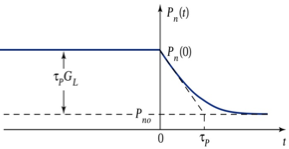
\includegraphics[width=0.7\columnwidth,keepaspectratio]{img/lightonoff.png}\eqbox{\tau_p = \frac{1}{\beta n_{n0}}}

    Light on:
    \begin{align*}
      G_L &= U = \frac{p_n-p_{n0}}{\tau_p} & p_n(t \leq 0) &= p_{n0} + \tau_pG_L
    \end{align*}

    Light off:
    \begin{align*}
      \Abl{p_n}{t} &= G_{th} - R = -U = -\frac{p_n-p_{n0}}{\tau_p} \\
      p_n(t) &= p_{n0} + \tau_p G_L \exp\left(-\frac{t}{\tau_p}\right)
    \end{align*}

    Generally:
    \eqbox{\Delta n = \tau_{n_0}R_n}

  \subsection{Indirect Generation/Recombination}
    \cgraphic{0.7}{img/trap.png}
    Energy trap near midgap.
    \[ U \approx  \frac{v_{th}\sigma_0N_t\cdot\Delta p}{1 + \frac{2n_i}{n_{n0}}\cosh\frac{E_t - E_i}{kT}} \approx \frac{\Delta p}{\tau_p} \approx \frac{p_n - p_{n0}}{\tau_p}\]
    Where $N_tv_{th}\sigma$ are the recombination events taking place per unit time, $v_{th}\sigma$ a cylindrical colume in material per unit time.
    \[\frac{1}{2}m_nv_{th}^2=\frac{3}{2}kT \quad v_{th}\approx 10^7 cm\cdot s^{-1}\]
    Electron capture ($R_a$) and emission ($R_b$) rate must be equal in therm. equi.
    \[R_a = nN_t(1-f)\cdot v_{th}\sigma_n \quad R_b = e_nN_tf\]
    The emission probability increases exponentially as $E_t$ gets closer to conduction band edge:
    \[e_n = \frac{v_{th}\sigma_nn(1-f)}{f}=v_{th}\sigma_nn_ie^{(E_t-E_i)/kT}\]
    For holes:
    \[R_c = pN_tf\cdot v_{th}\sigma_p \quad R_d = e_pN_t(1-f)\]
    \[e_p = v_{th}\sigma_p n_i e^{(E_i-E_t)/kT}\]
    These lead to the equation for $U=\dots$.

  \subsection{Diffusion}
    Result of concentration gradients.
    Equal probability of moving in any direction.
    Fick's first law of diffusion:
    \[J_{\text{diff}} = -D\Delta N = -D \left( \Pabl{N}{x}\vec{x_u} + \Pabl{N}{y}\vec{y_u} \dots \right)\]

    In thermal equi. and uniform distribution, free charge carriers are in constant motion. 
    Net current is thus zero.
    Statistical mechanics show that particles at temp. $T$ have avg. thermal energy of $3kT/2$
    For a particle of mass $m$ this corresponds to an avg. thermal velocity
    \[\frac{1}{2}mv_{th}^2=\frac{3}{2}kT\]
    In a crystal we must use the \textbf{effective mass}
    The electron diffusion current:
    \[ J_{\text{diff},n} = -qF = qD_n\Abl{n}{x}\]

  \subsection{Drift}
    Result of an electric field as driving force.
    Zero field: Electrons move thermally (randomly) in all directions (no net flow)
    Non-zero field: There is a net drift of electrons, opposite to the E-field
    We can then define a drift velocity of electrons $v_{dr,n}$
    Electrons do not accelerate indefinitely due to collisions
    \begin{align*}
      J_{dr,n} &= -qnv_{dr,n} & v_{dr,n} &= -\mu_nE \\
      J_{dr,p} &= qpv_{dr,h} & v_{dr,h} &= \mu_pE \\
      J_{dr,tot} &= \sigma E & \sigma &= q(n\mu_n + p\mu_p)
    \end{align*}
  
  \subsection{Total current}
    Total current = drift + diffusion current = electron + hole current.
    \begin{align*}
      &\text{Electrons:} & J_n &= nq\mu\vec{E}+qD_n\Abl{n}{x} \\
      &\text{Holes:} & J_p &= pq\mu\vec{E}-qD_p\Abl{p}{x} \\
    \end{align*}

  % ---------------------------------------------------------------------------
  \section{Excess Carriers}
  % ---------------------------------------------------------------------------
  % \subsection{Variables}
    \begin{tabular}[h]{l l}
      $G_{n/p}$   & Generation rate of el/hole \\
      $R_{n/p}$   & Recombination rate of el/hole \\
      $J_{n/p}$   & Current density of el/hole \\
      $L_{n/p}$   & Minority carrier diffusion length \\
      $D_{n/p}$   & Diffusion constant \\
      $\mu_{n/p}$ & Carrier mobility \\
    \end{tabular}

  \subsection{Continuity equation}
    \textbf{Objective:} Accounting for carrier densities when drift, diffusion and G/R take place.
    \cgraphic{0.5}{img/continuity.png}
    
    \begin{align*}
      &\text{Change in e} & \Pabl{n}{t} &= \frac{1}{q}\Pabl{J_n}{x}+(G_m-R_n) \\
      &\text{Change in hole} & \Pabl{p}{t} &= -\frac{1}{q}\Pabl{J_p}{x}+(G_p-R_p)
    \end{align*}

    Written for \textbf{electrons} in p-type material
    \begin{align*}
      \Pabl{n_p}{t} &= n_p\mu_n\Pabl{\vec{E}}{x}+\mu_n\vec{E}\Pabl{n_p}{x} + D_n\Pablq{n_p}{x} \\ &+ G_n - \frac{n_p-n_{p0}}{\tau_n}
    \end{align*}

    Written for \textbf{holes} in n-type material
    \begin{align*}
      \Pabl{p_n}{t} &= p_n\mu_p\Pabl{\vec{E}}{x}+\mu_p\vec{E}\Pabl{p_n}{x} + D_p\Pablq{p_n}{x} \\ &+ G_p - \frac{p_n-p_{n0}}{\tau_p}
    \end{align*}

    \subsubsection{Steady state}
    For steady state considerations:

    \ceqbox{0=D_n\Pablq{n_p}{x}+G_n-\frac{n_p-n_{p0}}{\tau_n}}
    
    \subsubsection{Einstein relation}
    \begin{center}
      \eqbox{D_p = \frac{kT}{q}\mu_p} \eqbox{D_n = \frac{kT}{q}\mu_n}
    \end{center}

    \subsubsection{Semi-infinite sample}
    \cgraphicd{0.49}{img/semiinf1.png}{img/semiinf2.png}
    \begin{align*}
      p(x) &= p_{n0} + (p_n(0)-p_{n0}) \exp\left(-\frac{x}{L_p}\right) \\
      L_p &= \sqrt{D_p\tau_p}
    \end{align*}

    \subsubsection{Finite sample}
    \cgraphicd{0.49}{img/finitesample1.png}{img/finitesample2.png}
    \begin{align*}
      p_n(x) &= p_{n0} + (p_n(0)-p_{n0}) \frac{\sinh\left(\frac{W-x}{L_p}\right)}{\sinh\left(\frac{W}{L_p}\right)}
    \end{align*}

    If $W \ll L_p$ then recombination is weak, few holes recombine in the time required for them to cross the region $W$.
    The excess carrier profile bebomes linear:
    \[p_n(x) = (p_n(0)-P_{n0})\frac{W-x}{W}\]

    % \begin{align*}

    % \end{align*}
    % \begin{align*}

    % \end{align*}


  \subsection{Equilibrium: constant fermi level}
  \cgraphic{0.5}{img/pnfermilevel.png}
  In equilibrium, the Fermi level mus be constant to balance transfer rates so that no net current flows.
  \ceqbox{E_{F1} = E_{F2}}


  \subsection{Doping: Band bending}
  Near the transition region, the distance between the Fermi level and conducition/valence band edge changes.
  Far away from the junction, the material does not ``know'' there is a junction.



\end{multicols*}

\setcounter{secnumdepth}{2}
\end{document}
